\paragraph{Ausgangssignale}
Es wurden insgesamt vier unterschiedliche Aufnahmen als Testsignale herangezogen. Davon wurden zwei Aufnahmen im B-Format synthetisch erzeugt, um auch sehr gerichtete Signale vergleichen zu können:

\begin{itemize}
	\item Synthetisches Zirpen mit Elevationswinkel $0^{\circ}$, rotierend in Azimuth mit Winkelgeschwindigkeit $90^{\circ}/s$
	\item Synthetisches Zirpen mit Elevationswinkel $0^{\circ}$, rotierend in Azimuth mit Winkelgeschwindigkeit $90^{\circ}/s$, nachträglich verhallt mittels FDN-Plugin
	\item Live-Musik Aufnahme mit Besetzung:
	\begin{itemize}
	  \item Schlagzeug
	  \item E-Bass
	  \item Cello
	  \item Piano
	\end{itemize}
	\item Umgebungsgeräusche Straßenkreuzung
\end{itemize}

Die synthetischen Signale wurden dabei mit Hilfe eines weiteren Skriptes in Octave produziert. Das zusätzlich verhallte Signal wurde in Reaper mit dem FDN Reverb Plugin aus der IEM Plugin Suite\footnote{IEM Plugin Suite: \url{https://plugins.iem.at/}} nachträglich bearbeitet. Dies soll einen direkteren Vergleich der Performance von stark gerichtetem und stark diffusem Signal bieten. Die Live-Musik Aufnahme wurde im IEM Cube angefertigt und bietet einen ausgeprägten räumlichen Eindruck, wobei die Ambience-Aufnahme an einer Straßenkreuzung die größte Diffusität aufweist. Diese Aufnahmen wurden mit Soundfield Mikrofonen durchgeführt. Somit werden im Hörversuch vier sehr unterschiedliche Aufnahmeszenarien verwendet.


\paragraph{Verglichene Kombinationen von Dekorrelation und Dekodierung}

Die folgende Liste zeigt die verglichenen Kombinationen aus Upmixing-, Dekorrelations- und Dekodierungsmethoden:

\begin{itemize}
	\item LSDecorr: DirAC, 12 Lautsprecher + Random Phase Decorrelation
	\item LSFDN: DirAC, 12 Lautsprecher + FDN Decorrelation
	\item TdesFDN: DirAC, t-Design + FDN Decorrelation
	\item TdesWid: DirAC, t-Design + Widening Plugin
	\item HARPEX\footnote{HARPEX: \url{https://harpex.net/index.html}}
	\item COMPASS\footnote{COMPASS: \url{http://research.spa.aalto.fi/projects/compass_vsts/plugins.html}}
\end{itemize}




Abbildung ~\ref{fig:algos} ist eine schematische Darstellung der Wiedergabe der Testsignale. Die Wiedergabe ist grundsätzlich immer eine Kombination aus vorhergehender Erzeugung und Bearbeitung in einem Octave-Skript, und Wiedergabe und Bearbeitung in Reaper mittels Plugins.

\begin{figure}[!ht]
  \centering
  
\includegraphics[width=1\textwidth]{aufbau/diagram.png}
  \caption{Flussdiagram Wiedergabe im Produktionsstudio}
  	\label{fig:algos}
\end{figure}

Die Dekodierung der ambisonischen Signale wird für alle Signale in GNU Octave durchgeführt. Nach dem DirAC-Upmixing wird die Dekodierung entweder auf die 12-Lautsprecher-Anordnung des Produktionsstudios, oder allgemein für ein 9-Design ausgeführt. Daher können die 12-Lautsprecher-dekodierten Signale in Reaper anschließend direkt auf die Lautsprecher ausgerichtet wiedergegeben werden, und das t-Design-Signal wird zuvor noch mit einem Dekodierungsplugin auf die Lautsprecher aufgeteilt.

\paragraph{Wiedergabesystem}
Als Wiedergabesytem wurde die Lautsprecheranordnung des Produktionsstudios des IEM verwendet. Prinzipiell besteht die Lautsprecheranordnung im Produktionsstudio aus zwei übereinander liegenden horizontalen Ringen und einem Zenit-Lautsprecher. Es werden insgesamt 12 Lautsprecher verwendet, jedoch befinden sich keine Lautsprecher in vertikaler Richtung unter dem Horizont. Eine Visualisierung der Lautsprecheranordnung ist in Abb. ~\ref{fig:aufb:prodstud} dargestellt. Der Nadir-Lautsprecher in der Abbildung ist ein imaginärer Lautsprecher um Signale unter dem Horizont auf andere Lautsprecher zu verteilen.

\begin{figure}[!ht]
  \centering
  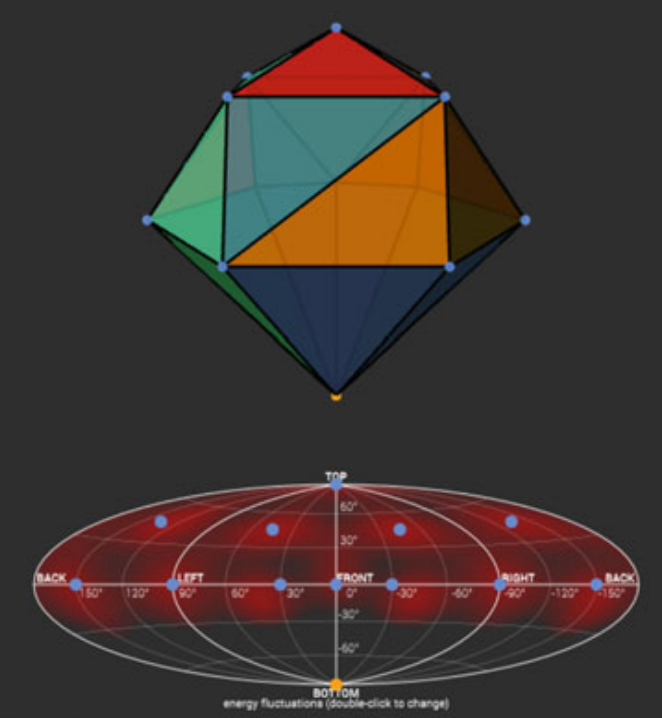
\includegraphics[width=0.4\textwidth]{aufbau/plots/speaker_pos_prod_studio.png}
  \caption{Visualisierung der Lautsprecheranordnung im Produktionsstudio des IEM aus \cite{ambi-book}}
  \label{fig:aufb:prodstud}
\end{figure}



Im Falle unseres Hörversuchs muss unbedingt angemerkt werden, dass der Center-Lautsprecher im horizontalen Ring fehlte. Dies führt natürlich zu einer schlechteren Lokalisierbarkeit und höheren Quellbreite an dieser Stelle. Da dieses Verhalten bei allen Algorithmen und für alle Versuchspersonen gleich war, wurde der Hörversuch jedoch trotzdem durchgeführt.

\paragraph{Versuchsinterface}
Um die Antworten der Versuchspersonen auszuwerten wurde eine Anwendung eingesetzt, die einen MUSHRA-Test realisiert (MUltiple Stimuli with Hidden Reference and Anchor). Diese Anwendung wird über eine \textit{.json}-Datei konfiguriert und kann als Steuerung für die Reaper DAW verwendet werden. Die Anwendung teilt die Zeitspur der DAW in \textit{scenes} auf. Unterschiedliche Klangbeispiele werden daher als Marker zeitlich geordnet. Die verglichenen Algorithmen werden als Spuren in der DAW gesteuert. Schaltet man einen Algorithmus ein, um ihn hörbar zu machen, wird also ein Regler einer Spur in Reaper auf 0dB aufgezogen. Die FOA-Referenz wurde in den getesteten Algorithmen ebenfalls inkludiert.

Die MUSHRA-Anwendung stellt alle Algorithmen in randomisierter Reihenfolge auf einer eigenen Seite für jede Szene (Klangbeispiel) dar. Dadurch kann die Versuchsperson bei einem Hörbeispiel alle möglichen Algorithmen vergleichen und mit Schiebereglern auf einer quasi-kontinuierlichen Skala bewerten. Wenn eine Szene bewertet wurde kann die Versuchsperson zur nächsten wechseln.
